\chapter{THIẾT KẾ MỨC QUAN NIỆM}
\section{Liệt kê và mô tả chức năng, ý nghĩa của các thực thể}

\begin{longtable}{|L{0.27\textwidth}|L{0.32\textwidth}|L{0.3\textwidth}|}
\hline
\textbf{Thực thể} & \textbf{Chức năng} & \textbf{Ý nghĩa} \\ \hline
\endfirsthead
\hline
\textbf{Thực thể} & \textbf{Chức năng} & \textbf{Ý nghĩa} \\ \hline
\endhead
ROLE & Lưu trữ các vai trò (quyền hạn) có thể gán cho người dùng trong hệ thống. & Là cơ sở để phân quyền, đảm bảo mỗi người dùng chỉ thực hiện đúng chức năng phù hợp với vai trò được gán. \\ \hline
USER & Lưu thông tin định danh, đăng nhập của người dùng. & Là chủ thể chính thực hiện các thao tác trong hệ thống như xử lý ticket, ghi audit log. \\ \hline
USER\_ROLE & Liên kết nhiều-nhiều giữa USER và ROLE. & Cho phép một người dùng có nhiều vai trò và một vai trò được áp dụng cho nhiều người dùng, tăng tính linh hoạt trong phân quyền. \\ \hline
SITE & Lưu thông tin địa điểm/cơ sở đặt Data Center. & Là cấp cao nhất trong cấu trúc hạ tầng vật lý, giúp quản lý theo khu vực địa lý. \\ \hline
ROOM & Lưu thông tin phòng thuộc một Site. & Chia nhỏ Site thành các phòng cụ thể để dễ quản lý vị trí đặt thiết bị. \\ \hline
RACK & Lưu thông tin tủ rack đặt server trong phòng. & Xác định vị trí vật lý chính xác của từng server, hỗ trợ vận hành và bảo trì. \\ \hline
SERVER & Lưu thông tin máy chủ vật lý (tên, IP, hệ điều hành, trạng thái...). & Là thực thể trung tâm của hệ thống, liên kết với hầu hết các module giám sát, cảnh báo, bảo hành. \\ \hline
CONTAINER & Lưu thông tin container/workload chạy trên server. & Phản ánh khối lượng công việc thực tế mà server đang xử lý. \\ \hline
WARRANTY & Lưu thông tin bảo hành của server. & Giúp theo dõi thời hạn bảo hành, hỗ trợ quyết định bảo trì hoặc thay thế thiết bị. \\ \hline
TELEMETRY & Lưu dữ liệu giám sát (CPU, RAM, Disk, Network, nhiệt độ) theo thời gian. & Là nguồn dữ liệu để phát hiện bất thường và đánh giá hiệu năng hoạt động của server. \\ \hline
ALERT\_THRESHOLD & Lưu ngưỡng cảnh báo được cấu hình cho từng chỉ số giám sát. & Là điều kiện để hệ thống tự động phát sinh Alert khi dữ liệu vượt ngưỡng. \\ \hline
ALERT & Lưu thông tin cảnh báo bất thường của server. & Là tín hiệu đầu tiên cho biết có sự cố tiềm ẩn, làm cơ sở để tạo Incident. \\ \hline
INCIDENT & Lưu thông tin về sự cố cần xử lý chính thức. & Chuyển từ cảnh báo kỹ thuật sang một quy trình xử lý sự cố có tổ chức. \\ \hline
TICKET & Lưu thông tin công việc xử lý sự cố được giao cho người dùng. & Là công cụ theo dõi tiến độ và phân công trách nhiệm xử lý. \\ \hline
MAINTENANCE & Lưu lịch sử các hoạt động bảo trì gắn với ticket. & Ghi nhận kết quả xử lý thực tế, phục vụ tra cứu và đánh giá hiệu quả bảo trì. \\ \hline
AUDIT\_LOG & Lưu lịch sử hoạt động và các thay đổi quan trọng của người dùng trong hệ thống. & Đảm bảo tính minh bạch, hỗ trợ truy vết trách nhiệm khi có sự cố. \\ \hline
\end{longtable}

\section{Viết các thuộc tính cho thực thể}

\subsection{ROLE}
\begin{longtable}{|L{0.25\textwidth}|L{0.38\textwidth}|L{0.26\textwidth}|}
\hline
\textbf{Thuộc tính} & \textbf{Mô tả} & \textbf{Constraint} \\ \hline
\endfirsthead
\hline
\textbf{Thuộc tính} & \textbf{Mô tả} & \textbf{Constraint} \\ \hline
\endhead
role\_id & Mã định danh duy nhất của vai trò & PK \\ \hline
role\_name & Tên vai trò, ví dụ: Administrator, Operator, Technician & NOT NULL, UNIQUE \\ \hline
description & Mô tả chức năng hoặc quyền của vai trò & NULL \\ \hline
\end{longtable}

\subsection{USER}
\begin{longtable}{|L{0.25\textwidth}|L{0.38\textwidth}|L{0.26\textwidth}|}
\hline
\textbf{Thuộc tính} & \textbf{Mô tả} & \textbf{Constraint} \\ \hline
\endfirsthead
\hline
\textbf{Thuộc tính} & \textbf{Mô tả} & \textbf{Constraint} \\ \hline
\endhead
user\_id & Mã định danh duy nhất của người dùng & PK \\ \hline
username & Tên đăng nhập của người dùng & NOT NULL, UNIQUE \\ \hline
password\_hash & Mật khẩu đã được mã hóa & NOT NULL \\ \hline
full\_name & Họ và tên người dùng & NOT NULL \\ \hline
email & Địa chỉ email của người dùng & NOT NULL, UNIQUE \\ \hline
status & Trạng thái hoạt động của tài khoản & NOT NULL, DEFAULT 'Inactive' \\ \hline
\end{longtable}

\subsection{USER\_ROLE}
\begin{longtable}{|L{0.25\textwidth}|L{0.38\textwidth}|L{0.26\textwidth}|}
\hline
\textbf{Thuộc tính} & \textbf{Mô tả} & \textbf{Constraint} \\ \hline
\endfirsthead
\hline
\textbf{Thuộc tính} & \textbf{Mô tả} & \textbf{Constraint} \\ \hline
\endhead
user\_role\_id & Mã định danh duy nhất của bản ghi phân quyền & PK \\ \hline
user\_id\_fk & Mã người dùng & FK, NOT NULL \\ \hline
role\_id\_fk & Mã vai trò & FK, NOT NULL \\ \hline
UNIQUE(user\_id\_fk, role\_id\_fk) & Đảm bảo một vai trò không được gán trùng cho cùng một người dùng & UNIQUE \\ \hline
\end{longtable}

\subsection{SITE}
\begin{longtable}{|L{0.25\textwidth}|L{0.38\textwidth}|L{0.26\textwidth}|}
\hline
\textbf{Thuộc tính} & \textbf{Mô tả} & \textbf{Constraint} \\ \hline
\endfirsthead
\hline
\textbf{Thuộc tính} & \textbf{Mô tả} & \textbf{Constraint} \\ \hline
\endhead
site\_id & Mã định danh duy nhất của địa điểm & PK \\ \hline
site\_name & Tên địa điểm hoặc cơ sở & NOT NULL, UNIQUE \\ \hline
location & Địa chỉ hoặc vị trí vật lý của Site & NOT NULL \\ \hline
\end{longtable}

\subsection{ROOM}
\begin{longtable}{|L{0.25\textwidth}|L{0.38\textwidth}|L{0.26\textwidth}|}
\hline
\textbf{Thuộc tính} & \textbf{Mô tả} & \textbf{Constraint} \\ \hline
\endfirsthead
\hline
\textbf{Thuộc tính} & \textbf{Mô tả} & \textbf{Constraint} \\ \hline
\endhead
room\_id & Mã định danh duy nhất của phòng & PK \\ \hline
room\_name & Tên phòng hoặc khu vực & NOT NULL \\ \hline
site\_id\_fk & Mã Site mà phòng thuộc về & FK, NOT NULL \\ \hline
\end{longtable}

\subsection{RACK}
\begin{longtable}{|L{0.25\textwidth}|L{0.38\textwidth}|L{0.26\textwidth}|}
\hline
\textbf{Thuộc tính} & \textbf{Mô tả} & \textbf{Constraint} \\ \hline
\endfirsthead
\hline
\textbf{Thuộc tính} & \textbf{Mô tả} & \textbf{Constraint} \\ \hline
\endhead
rack\_id & Mã định danh duy nhất của Rack & PK \\ \hline
rack\_name & Tên hoặc mã nhận diện của Rack & NOT NULL \\ \hline
room\_id\_fk & Mã Room mà Rack thuộc về & FK, NOT NULL \\ \hline
\end{longtable}

\subsection{SERVER}
\begin{longtable}{|L{0.25\textwidth}|L{0.38\textwidth}|L{0.26\textwidth}|}
\hline
\textbf{Thuộc tính} & \textbf{Mô tả} & \textbf{Constraint} \\ \hline
\endfirsthead
\hline
\textbf{Thuộc tính} & \textbf{Mô tả} & \textbf{Constraint} \\ \hline
\endhead
server\_id & Mã định danh duy nhất của Server & PK \\ \hline
server\_name & Tên hoặc mã nhận diện của Server & NOT NULL, UNIQUE \\ \hline
ip\_address & Địa chỉ IP của Server & NOT NULL, UNIQUE \\ \hline
operating\_system & Hệ điều hành đang sử dụng trên Server & NOT NULL \\ \hline
status & Trạng thái hoạt động của Server & NOT NULL, DEFAULT 'Inactive' \\ \hline
rack\_id\_fk & Mã Rack mà Server được đặt trong & FK, NOT NULL \\ \hline
\end{longtable}

\subsection{CONTAINER}
\begin{longtable}{|L{0.25\textwidth}|L{0.38\textwidth}|L{0.26\textwidth}|}
\hline
\textbf{Thuộc tính} & \textbf{Mô tả} & \textbf{Constraint} \\ \hline
\endfirsthead
\hline
\textbf{Thuộc tính} & \textbf{Mô tả} & \textbf{Constraint} \\ \hline
\endhead
container\_id & Mã định danh duy nhất của Container & PK \\ \hline
container\_name & Tên hoặc mã nhận diện của Container & NOT NULL \\ \hline
container\_type & Loại Container hoặc Workload & NULL \\ \hline
status & Trạng thái hoạt động của Container & NOT NULL, DEFAULT 'Inactive' \\ \hline
server\_id\_fk & Mã Server mà Container đang chạy trên & FK, NOT NULL \\ \hline
\end{longtable}

\subsection{WARRANTY}
\begin{longtable}{|L{0.25\textwidth}|L{0.38\textwidth}|L{0.26\textwidth}|}
\hline
\textbf{Thuộc tính} & \textbf{Mô tả} & \textbf{Constraint} \\ \hline
\endfirsthead
\hline
\textbf{Thuộc tính} & \textbf{Mô tả} & \textbf{Constraint} \\ \hline
\endhead
warranty\_id & Mã định danh duy nhất của thông tin bảo hành & PK \\ \hline
provider & Nhà cung cấp hoặc đơn vị bảo hành & NOT NULL \\ \hline
warranty\_start & Ngày bắt đầu bảo hành & NOT NULL \\ \hline
warranty\_end & Ngày kết thúc bảo hành & NOT NULL \\ \hline
status & Trạng thái bảo hành & NOT NULL \\ \hline
server\_id\_fk & Mã Server được bảo hành & FK, NOT NULL, UNIQUE \\ \hline
\end{longtable}

\subsection{TELEMETRY}
\begin{longtable}{|L{0.25\textwidth}|L{0.38\textwidth}|L{0.26\textwidth}|}
\hline
\textbf{Thuộc tính} & \textbf{Mô tả} & \textbf{Constraint} \\ \hline
\endfirsthead
\hline
\textbf{Thuộc tính} & \textbf{Mô tả} & \textbf{Constraint} \\ \hline
\endhead
telemetry\_id & Mã định danh duy nhất của bản ghi Telemetry & PK \\ \hline
cpu\_usage & Mức sử dụng CPU của Server tại thời điểm ghi nhận & NOT NULL \\ \hline
ram\_usage & Mức sử dụng RAM của Server tại thời điểm ghi nhận & NOT NULL \\ \hline
disk\_usage & Mức sử dụng dung lượng Disk tại thời điểm ghi nhận & NOT NULL \\ \hline
network\_usage & Mức sử dụng hoặc lưu lượng mạng tại thời điểm ghi nhận & NULL \\ \hline
temperature & Nhiệt độ của Server tại thời điểm ghi nhận & NULL \\ \hline
recorded\_at & Thời điểm dữ liệu được ghi nhận & NOT NULL \\ \hline
server\_id\_fk & Mã Server tạo ra dữ liệu Telemetry & FK, NOT NULL \\ \hline
\end{longtable}

\subsection{ALERT\_THRESHOLD}
\begin{longtable}{|L{0.25\textwidth}|L{0.38\textwidth}|L{0.26\textwidth}|}
\hline
\textbf{Thuộc tính} & \textbf{Mô tả} & \textbf{Constraint} \\ \hline
\endfirsthead
\hline
\textbf{Thuộc tính} & \textbf{Mô tả} & \textbf{Constraint} \\ \hline
\endhead
threshold\_id & Mã định danh duy nhất của ngưỡng cảnh báo & PK \\ \hline
metric\_name & Tên chỉ số được giám sát, ví dụ: CPU, RAM, Disk & NOT NULL \\ \hline
warning\_value & Ngưỡng cảnh báo mức Warning & NOT NULL \\ \hline
critical\_value & Ngưỡng cảnh báo mức Critical & NOT NULL \\ \hline
is\_active & Trạng thái áp dụng của ngưỡng & NOT NULL, DEFAULT 1 \\ \hline
server\_id\_fk & Mã Server áp dụng ngưỡng cảnh báo & FK, NOT NULL \\ \hline
\end{longtable}

\subsection{ALERT}
\begin{longtable}{|L{0.25\textwidth}|L{0.38\textwidth}|L{0.26\textwidth}|}
\hline
\textbf{Thuộc tính} & \textbf{Mô tả} & \textbf{Constraint} \\ \hline
\endfirsthead
\hline
\textbf{Thuộc tính} & \textbf{Mô tả} & \textbf{Constraint} \\ \hline
\endhead
alert\_id & Mã định danh duy nhất của cảnh báo & PK \\ \hline
alert\_type & Loại cảnh báo, ví dụ: High CPU, High RAM, Disk Full & NOT NULL \\ \hline
severity & Mức độ nghiêm trọng của cảnh báo & NOT NULL \\ \hline
description & Mô tả chi tiết về cảnh báo & NULL \\ \hline
status & Trạng thái xử lý cảnh báo & NOT NULL, DEFAULT 'OPEN' \\ \hline
created\_at & Thời điểm cảnh báo được tạo & NOT NULL \\ \hline
server\_id\_fk & Mã Server phát sinh cảnh báo & FK, NOT NULL \\ \hline
\end{longtable}

\subsection{INCIDENT}
\begin{longtable}{|L{0.25\textwidth}|L{0.38\textwidth}|L{0.26\textwidth}|}
\hline
\textbf{Thuộc tính} & \textbf{Mô tả} & \textbf{Constraint} \\ \hline
\endfirsthead
\hline
\textbf{Thuộc tính} & \textbf{Mô tả} & \textbf{Constraint} \\ \hline
\endhead
incident\_id & Mã định danh duy nhất của sự cố & PK \\ \hline
incident\_title & Tiêu đề hoặc tên của sự cố & NOT NULL \\ \hline
description & Mô tả chi tiết về sự cố & NULL \\ \hline
priority & Mức độ ưu tiên xử lý sự cố & NOT NULL \\ \hline
status & Trạng thái xử lý sự cố & NOT NULL, DEFAULT 'OPEN' \\ \hline
created\_at & Thời điểm Incident được tạo & NOT NULL \\ \hline
alert\_id\_fk & Mã Alert liên quan đến Incident & FK, NOT NULL \\ \hline
\end{longtable}

\subsection{TICKET}
\begin{longtable}{|L{0.25\textwidth}|L{0.38\textwidth}|L{0.26\textwidth}|}
\hline
\textbf{Thuộc tính} & \textbf{Mô tả} & \textbf{Constraint} \\ \hline
\endfirsthead
\hline
\textbf{Thuộc tính} & \textbf{Mô tả} & \textbf{Constraint} \\ \hline
\endhead
ticket\_id & Mã định danh duy nhất của Ticket & PK \\ \hline
ticket\_title & Tiêu đề hoặc tên công việc cần thực hiện & NOT NULL \\ \hline
description & Mô tả chi tiết công việc cần xử lý & NULL \\ \hline
priority & Mức độ ưu tiên của Ticket & NOT NULL \\ \hline
status & Trạng thái xử lý Ticket & NOT NULL, DEFAULT 'OPEN' \\ \hline
created\_at & Thời điểm Ticket được tạo & NOT NULL \\ \hline
incident\_id\_fk & Mã Incident mà Ticket liên quan đến & FK, NOT NULL \\ \hline
assigned\_user\_id\_fk & Mã User được phân công xử lý Ticket & FK, NOT NULL \\ \hline
\end{longtable}

\subsection{MAINTENANCE}
\begin{longtable}{|L{0.25\textwidth}|L{0.38\textwidth}|L{0.26\textwidth}|}
\hline
\textbf{Thuộc tính} & \textbf{Mô tả} & \textbf{Constraint} \\ \hline
\endfirsthead
\hline
\textbf{Thuộc tính} & \textbf{Mô tả} & \textbf{Constraint} \\ \hline
\endhead
maintenance\_id & Mã định danh duy nhất của hoạt động bảo trì & PK \\ \hline
maintenance\_type & Loại hoạt động bảo trì hoặc xử lý được thực hiện & NOT NULL \\ \hline
description & Mô tả chi tiết về hoạt động bảo trì & NULL \\ \hline
performed\_at & Thời điểm thực hiện hoạt động bảo trì & NOT NULL \\ \hline
result & Kết quả sau khi thực hiện bảo trì & NULL \\ \hline
ticket\_id\_fk & Mã Ticket liên quan đến hoạt động bảo trì & FK, NOT NULL \\ \hline
\end{longtable}

\subsection{AUDIT\_LOG}
\begin{longtable}{|L{0.25\textwidth}|L{0.38\textwidth}|L{0.26\textwidth}|}
\hline
\textbf{Thuộc tính} & \textbf{Mô tả} & \textbf{Constraint} \\ \hline
\endfirsthead
\hline
\textbf{Thuộc tính} & \textbf{Mô tả} & \textbf{Constraint} \\ \hline
\endhead
audit\_log\_id & Mã định danh duy nhất của bản ghi nhật ký & PK \\ \hline
action & Hành động hoặc sự kiện được ghi nhận & NOT NULL \\ \hline
entity\_type & Loại thực thể hoặc đối tượng bị tác động & NOT NULL \\ \hline
entity\_id & Mã định danh của đối tượng liên quan & NULL \\ \hline
description & Mô tả chi tiết về hoạt động hoặc thay đổi & NULL \\ \hline
created\_at & Thời điểm hoạt động được ghi nhận & NOT NULL \\ \hline
user\_id\_fk & Mã User thực hiện hoạt động (nếu có) & FK, NULL \\ \hline
\end{longtable}

\section{Xác định các mối quan hệ giữa các thực thể}

\begin{longtable}{|L{0.05\textwidth}|L{0.13\textwidth}|L{0.12\textwidth}|L{0.15\textwidth}|L{0.44\textwidth}|}
\hline
\textbf{STT} & \textbf{Thực thể 1} & \textbf{Cardinality} & \textbf{Thực thể 2} & \textbf{Mô tả mối quan hệ} \\ \hline
\endfirsthead
\hline
\textbf{STT} & \textbf{Thực thể 1} & \textbf{Cardinality} & \textbf{Thực thể 2} & \textbf{Mô tả mối quan hệ} \\ \hline
\endhead
1 & USER & 1:N & USER\_ROLE & Một User có thể được gán nhiều Role thông qua nhiều bản ghi trong USER\_ROLE. \\ \hline
2 & ROLE & 1:N & USER\_ROLE & Một Role có thể được gán cho nhiều User thông qua nhiều bản ghi trong USER\_ROLE. \\ \hline
3 & SITE & 1:N & ROOM & Một Site có thể có nhiều Room, mỗi Room thuộc về một Site. \\ \hline
4 & ROOM & 1:N & RACK & Một Room có thể có nhiều Rack, mỗi Rack thuộc về một Room. \\ \hline
5 & RACK & 1:N & SERVER & Một Rack có thể chứa nhiều Server, mỗi Server được đặt trong một Rack. \\ \hline
6 & SERVER & 1:N & CONTAINER & Một Server có thể chạy nhiều Container, mỗi Container thuộc về một Server. \\ \hline
7 & SERVER & 1:0..1 & WARRANTY & Một Server có thể chưa có hoặc có một bản ghi bảo hành hiện tại; mỗi Warranty thuộc về một Server. \\ \hline
8 & SERVER & 1:N & TELEMETRY & Một Server có thể có nhiều bản ghi Telemetry theo thời gian. \\ \hline
9 & SERVER & 1:N & ALERT\_THRESHOLD & Một Server có thể được cấu hình nhiều ngưỡng cảnh báo cho các chỉ số khác nhau. \\ \hline
10 & SERVER & 1:N & ALERT & Một Server có thể phát sinh nhiều Alert trong quá trình hoạt động. \\ \hline
11 & ALERT & 1:0..1 & INCIDENT & Một Alert có thể không tạo Incident; nếu cần xử lý chính thức thì có thể tạo một Incident. \\ \hline
12 & INCIDENT & 1:N & TICKET & Một Incident có thể cần một hoặc nhiều Ticket để theo dõi và xử lý công việc. \\ \hline
13 & USER & 1:N & TICKET & Một User có thể được giao nhiều Ticket; mỗi Ticket được giao cho một User phụ trách. \\ \hline
14 & TICKET & 1:N & MAINTENANCE & Một Ticket có thể có nhiều hoạt động hoặc bản ghi Maintenance. \\ \hline
15 & USER & 1:N & AUDIT\_LOG & Một User có thể tạo hoặc thực hiện nhiều hoạt động được ghi nhận trong AUDIT\_LOG. \\ \hline
\end{longtable}

\section{BUSINESS RULES CỦA NHÓM THỰC THỂ}

\subsection{Quy tắc nghiệp vụ về quản lý người dùng và phân quyền}
\begin{longtable}{|L{0.23\textwidth}|L{0.66\textwidth}|}
\hline
\textbf{Mã quy tắc} & \textbf{Nội dung} \\ \hline
\endfirsthead
\hline
\textbf{Mã quy tắc} & \textbf{Nội dung} \\ \hline
\endhead
BR-UM-01 & Mỗi người dùng trong hệ thống phải được xác định bằng một mã định danh duy nhất. \\ \hline
BR-UM-02 & Mỗi người dùng phải có tên đăng nhập duy nhất để phục vụ cho việc xác thực và truy cập hệ thống. \\ \hline
BR-UM-03 & Mỗi người dùng có thể được gán một hoặc nhiều vai trò trong hệ thống. \\ \hline
BR-UM-04 & Mỗi vai trò có thể được gán cho nhiều người dùng khác nhau. \\ \hline
BR-UM-05 & Mối quan hệ giữa người dùng và vai trò được quản lý thông qua thực thể USER\_ROLE. \\ \hline
BR-UM-06 & Mỗi bản ghi trong USER\_ROLE phải tham chiếu đến một người dùng và một vai trò hợp lệ. \\ \hline
BR-UM-07 & Một người dùng chỉ có thể thực hiện các chức năng phù hợp với vai trò được phân quyền. \\ \hline
\end{longtable}

\subsection{Quy tắc nghiệp vụ về quản lý hạ tầng và tài sản}
\begin{longtable}{|L{0.23\textwidth}|L{0.66\textwidth}|}
\hline
\textbf{Mã quy tắc} & \textbf{Nội dung} \\ \hline
\endfirsthead
\hline
\textbf{Mã quy tắc} & \textbf{Nội dung} \\ \hline
\endhead
BR-INF-01 & Một Site có thể bao gồm nhiều Room, nhưng mỗi Room chỉ thuộc về một Site. \\ \hline
BR-INF-02 & Một Room có thể bao gồm nhiều Rack, nhưng mỗi Rack chỉ thuộc về một Room. \\ \hline
BR-INF-03 & Một Rack có thể chứa nhiều Server, nhưng mỗi Server chỉ được đặt trong một Rack tại một thời điểm. \\ \hline
BR-INF-04 & Mỗi Server phải được xác định bằng một mã định danh duy nhất. \\ \hline
BR-INF-05 & Thông tin vị trí của Server được xác định dựa trên cấu trúc phân cấp: Site $\rightarrow$ Room $\rightarrow$ Rack $\rightarrow$ Server. \\ \hline
BR-INF-06 & Một Server có thể vận hành một hoặc nhiều Container. \\ \hline
BR-INF-07 & Mỗi Container phải thuộc về một Server xác định. \\ \hline
BR-INF-08 & Thông tin bảo hành được sử dụng để theo dõi thời gian và tình trạng bảo hành của Server. \\ \hline
BR-INF-09 & Mỗi bản ghi Warranty phải được liên kết với một Server hợp lệ. \\ \hline
BR-INF-10 & Thông tin bảo hành có thể được sử dụng để hỗ trợ theo dõi các Server còn hiệu lực hoặc sắp hết hạn bảo hành. \\ \hline
\end{longtable}

\subsection{Quy tắc nghiệp vụ về giám sát hệ thống}
\begin{longtable}{|L{0.23\textwidth}|L{0.66\textwidth}|}
\hline
\textbf{Mã quy tắc} & \textbf{Nội dung} \\ \hline
\endfirsthead
\hline
\textbf{Mã quy tắc} & \textbf{Nội dung} \\ \hline
\endhead
BR-MON-01 & Dữ liệu Telemetry phải được ghi nhận cho một Server xác định. \\ \hline
BR-MON-02 & Một Server có thể có nhiều bản ghi Telemetry theo thời gian. \\ \hline
BR-MON-03 & Mỗi bản ghi Telemetry phải bao gồm thời điểm ghi nhận để hỗ trợ theo dõi lịch sử hoạt động của Server. \\ \hline
BR-MON-04 & Dữ liệu Telemetry có thể bao gồm các thông số giám sát như mức sử dụng CPU, RAM, dung lượng lưu trữ, lưu lượng mạng và nhiệt độ. \\ \hline
BR-MON-05 & Các cấu hình ngưỡng cảnh báo (Alert Threshold) được sử dụng để xác định điều kiện bất thường của các thông số giám sát. \\ \hline
BR-MON-06 & Một Server có thể có một hoặc nhiều cấu hình ngưỡng cảnh báo cho các chỉ số giám sát khác nhau. \\ \hline
BR-MON-07 & Mỗi cấu hình ngưỡng cảnh báo phải được liên kết với một Server xác định. \\ \hline
BR-MON-08 & Khi một thông số giám sát vượt quá ngưỡng đã được thiết lập, hệ thống có thể tạo một Alert tương ứng. \\ \hline
BR-MON-09 & Mỗi Alert phải được liên kết với một Server xác định. \\ \hline
BR-MON-10 & Một Server có thể phát sinh nhiều Alert trong quá trình hoạt động. \\ \hline
BR-MON-11 & Mỗi Alert được tạo ra phải lưu thông tin liên quan đến loại cảnh báo, giá trị hoặc điều kiện gây cảnh báo, trạng thái và thời điểm tạo. \\ \hline
\end{longtable}

\subsection{Quy tắc nghiệp vụ về cảnh báo và xử lý sự cố}
\begin{longtable}{|L{0.23\textwidth}|L{0.66\textwidth}|}
\hline
\textbf{Mã quy tắc} & \textbf{Nội dung} \\ \hline
\endfirsthead
\hline
\textbf{Mã quy tắc} & \textbf{Nội dung} \\ \hline
\endhead
BR-IM-01 & Mỗi Alert phải được liên kết với một Server xác định. \\ \hline
BR-IM-02 & Một Server có thể phát sinh nhiều Alert trong quá trình hoạt động. \\ \hline
BR-IM-03 & Mỗi Alert được tạo ra phải lưu thông tin liên quan đến loại cảnh báo, giá trị hoặc điều kiện gây cảnh báo, trạng thái và thời điểm tạo. \\ \hline
BR-IM-04 & Một Alert cần được xử lý có thể dẫn đến việc tạo một Incident. \\ \hline
BR-IM-05 & Mỗi Incident phải được liên kết với Alert đã gây ra hoặc liên quan đến sự cố đó. \\ \hline
BR-IM-06 & Một Incident có thể được sử dụng làm cơ sở để tạo một hoặc nhiều Ticket xử lý. \\ \hline
BR-IM-07 & Mỗi Ticket phải được liên kết với một Incident xác định. \\ \hline
BR-IM-08 & Một Ticket có thể được phân công cho một người dùng phù hợp để thực hiện việc xử lý. \\ \hline
BR-IM-09 & Người dùng được phân công xử lý Ticket phải tồn tại trong hệ thống. \\ \hline
BR-IM-10 & Trạng thái của Ticket phải được cập nhật theo quá trình xử lý sự cố. \\ \hline
\end{longtable}

\subsection{Quy tắc nghiệp vụ về bảo trì}
\begin{longtable}{|L{0.23\textwidth}|L{0.66\textwidth}|}
\hline
\textbf{Mã quy tắc} & \textbf{Nội dung} \\ \hline
\endfirsthead
\hline
\textbf{Mã quy tắc} & \textbf{Nội dung} \\ \hline
\endhead
BR-MT-01 & Hoạt động bảo trì được thực hiện dựa trên các Ticket cần được xử lý. \\ \hline
BR-MT-02 & Mỗi bản ghi Maintenance phải được liên kết với một Ticket xác định. \\ \hline
BR-MT-03 & Một Ticket có thể có một hoặc nhiều hoạt động bảo trì tùy thuộc vào quá trình xử lý. \\ \hline
BR-MT-04 & Thông tin Maintenance cần lưu lại loại hoạt động bảo trì, mô tả công việc, thời điểm thực hiện và kết quả thực hiện. \\ \hline
BR-MT-05 & Các hoạt động bảo trì được lưu trữ nhằm hỗ trợ theo dõi lịch sử sửa chữa và bảo trì của hệ thống. \\ \hline
\end{longtable}

\subsection{Quy tắc nghiệp vụ về nhật ký hoạt động}
\begin{longtable}{|L{0.23\textwidth}|L{0.66\textwidth}|}
\hline
\textbf{Mã quy tắc} & \textbf{Nội dung} \\ \hline
\endfirsthead
\hline
\textbf{Mã quy tắc} & \textbf{Nội dung} \\ \hline
\endhead
BR-AU-01 & Các hoạt động quan trọng trong hệ thống có thể được ghi nhận vào AUDIT\_LOG. \\ \hline
BR-AU-02 & Mỗi bản ghi Audit Log phải lưu thông tin về hành động được thực hiện và thời điểm thực hiện. \\ \hline
BR-AU-03 & Một người dùng có thể thực hiện nhiều hoạt động khác nhau trong hệ thống. \\ \hline
BR-AU-04 & Một người dùng có thể có nhiều bản ghi trong AUDIT\_LOG, nhưng mỗi bản ghi Audit Log chỉ liên kết với một người dùng thực hiện hành động. \\ \hline
\end{longtable}

\section{ERD}

Sơ đồ ERD tổng thể được xây dựng dựa trên các thực thể, thuộc tính và mối quan hệ đã xác định ở các phần trên. Sơ đồ thể hiện cấu trúc cơ sở dữ liệu AR-IMMS và các liên kết giữa các thực thể.

Các nhóm quan hệ chính trong ERD gồm: ROLE -- USER -- USER\_ROLE; SITE -- ROOM -- RACK -- SERVER -- CONTAINER; SERVER -- WARRANTY; SERVER -- TELEMETRY; SERVER -- ALERT\_THRESHOLD -- ALERT; ALERT -- INCIDENT -- TICKET; USER -- TICKET; TICKET -- MAINTENANCE; và USER -- AUDIT\_LOG.

\begin{figure}[htbp]
    \centering
    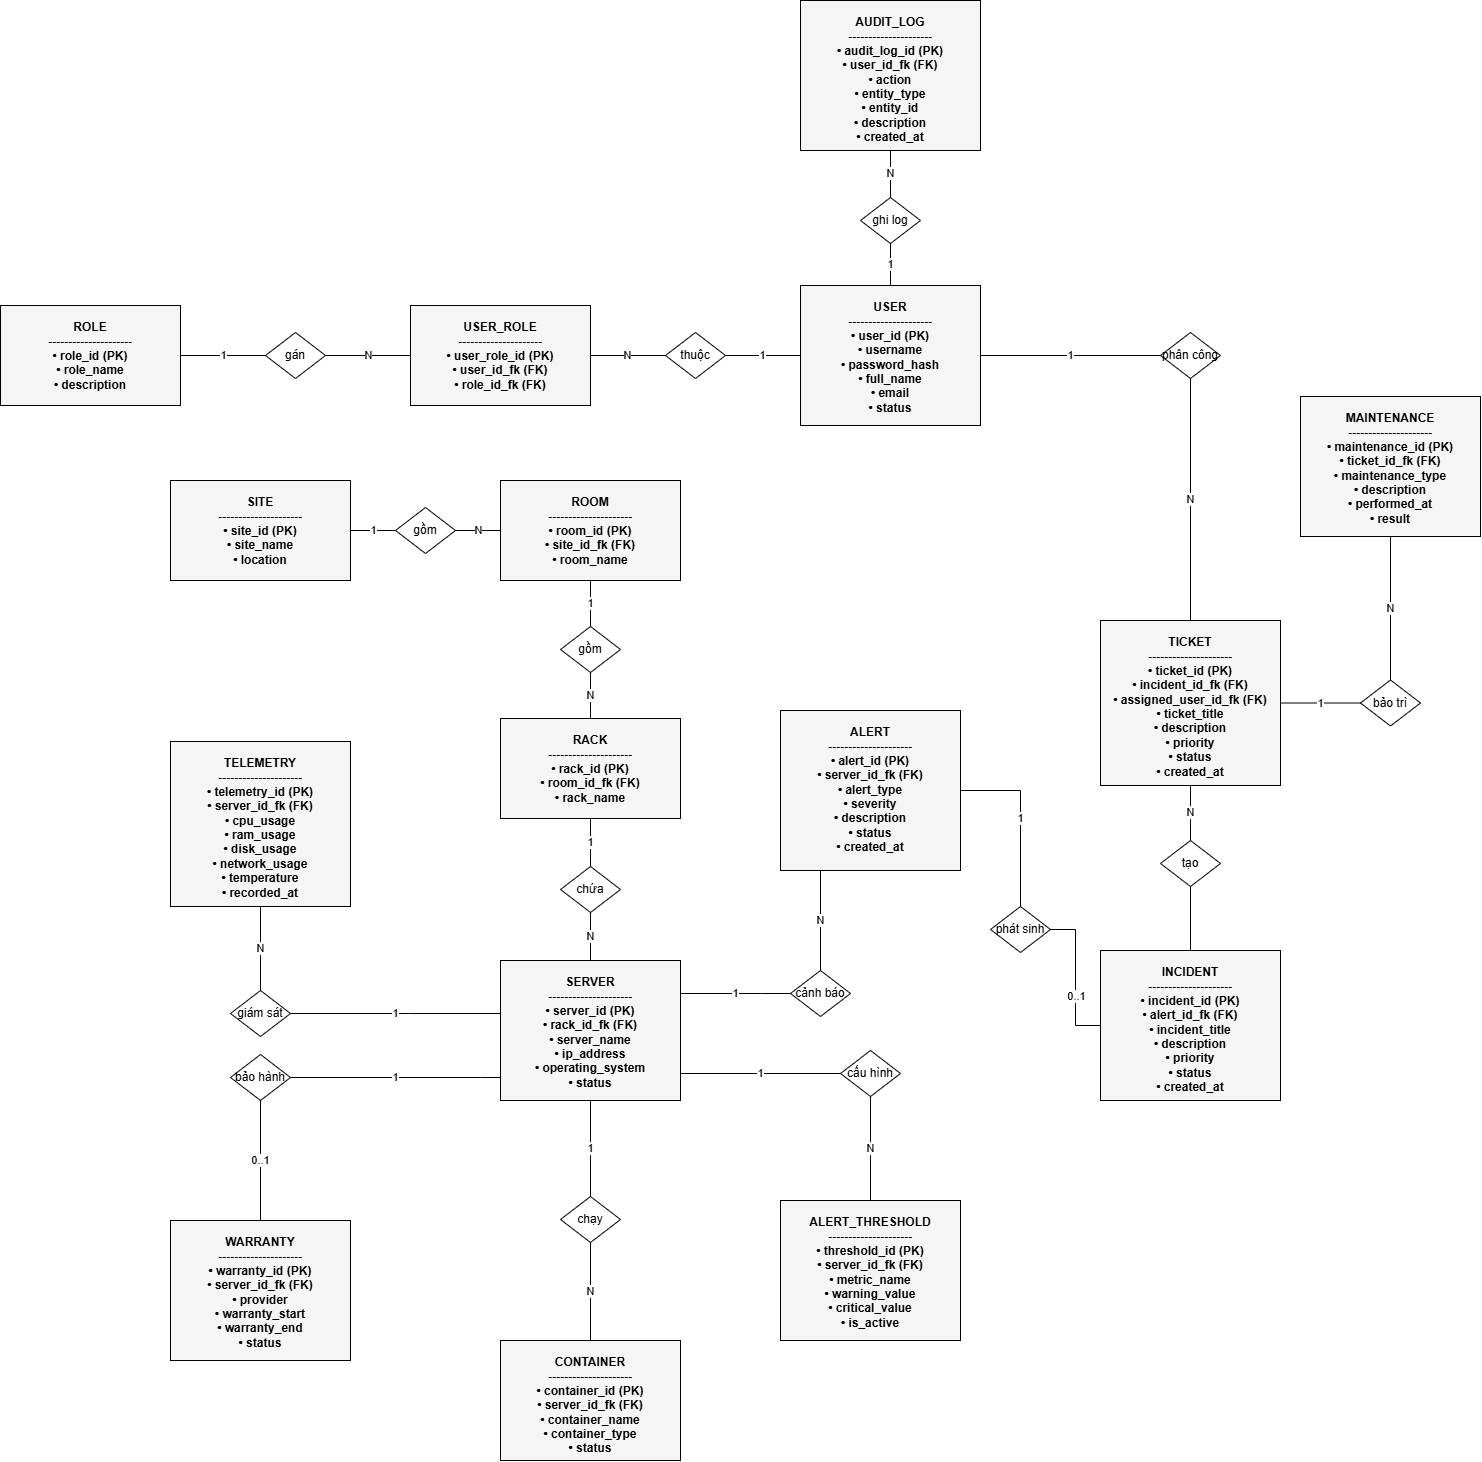
\includegraphics[width=\textwidth,height=0.68\textheight,keepaspectratio]{ERD.drawio.png}
    \caption{Sơ đồ ERD tổng thể của cơ sở dữ liệu AR-IMMS.}
    \label{fig:erd_chuong2}
\end{figure}
